\newpage
\chapter{Реализация}\label{ch:chapter_2}

\section{Middleware For Collaboration Implementation}

There is a lot of ways to achieve network communication between applications
starting from assembling raw TCP/IP datagrams up to using object-oriented
libraries for specific application-level protocols. We stated a list of
requirements to choose an appropriate middleware technology. These requirements
were collected from the three sources: our view of collaboration, restrictions
imposed by the target platforms and a preliminary architecture of the
application.

According to our view of collaboration (see section \ref{})
we have a server and several clients. For the sake of simplicity we assume that a server is allowed to be created anytime. Clients connect to server and modify
the shared mind map. Every change of the map is propagated via the server, which
notifies all the clients about it. For robust communicating all the participants
must always have the exact copy of the mind map.

HiveMind is now targeted at both mobile devices and PCs. Each platform gives us
unique advantages. PC users usually have wide broadband Internet
connection. Mobile devices can gain Internet access almost anytime and
anywhere. Due to the lack of IPv4 addresses mobile operators often assign
private IP addresses to mobile devices that makes them unreachable from the
Internet. Data transmission via wireless media sometimes causes unreasonable
delays for several seconds or more. PC users can use NAT or complex firewall
software that blocks incoming connections. It may be even worse: in corporate
environments users are often limited to HTTP proxy as the only source of the
Internet connection.

Summarizing all these challenges we get the following list of requirements for
middleware technology.
\begin{itemize}
\item Communication is based on the client-server model.
\item Server supports for subscription.
\item Users may have a slow unreliable connection to the Internet through the
  NAT gateway.
\item There must be no additional effort to set up the server.
\item Middleware must be supported by a Python library.
\end{itemize}

%This is not full list of requirements. It can be filled up with these
%statements. They cover additional functionality.
%\begin{itemize}
%\item Technology should support transient or backup server to reinforce
%communication between nodes.
%\item Messages may be encrypted to ensure the privacy of shared map.
%\item Technology should support instant messaging system.
%\end{itemize}

We compared several alternative technologies and chose the XMPP protocol as it
allows us to avoid almost all concerns about implementation of client-server
communication.

XMPP protocol can be considered at the several levels of abstraction. At the low
level there is a XMPP client application that connects to the XMPP server and
exchanges messages with it. Connection can be established in many ways, even on
top of HTTP protocol. At the higher level of abstraction the client gains access
to the whole network, where every node has unique identifier (JID) and no
additional effort required to exchange information between them. The client
creates a message addressed to another client and sends it to the server, which
handles all the routine to deliver the message.

Another great feature of XMPP is protocol extensions (XEP). 
XMPP is an open protocol and anyone may create a custom high-level protocol on
top of it. XMPP Standards Foundation manages the process of creation and
maintenance of such protocols. There is XEP-0060 Publish-Subscribe extension
\cite{xep-0060}. It defines how to implement publish/subscribe services on top
of XMPP. Any member of the network can create pub/sub service. XMPP protocol
with Publish-Subscribe extension fits the best into our requirements and that is
why it is our choice for middleware technology.

XMPP protocol is XML-based, and it may seem that using this protocol would
require broadband Internet connection, but it is not so. Intercommunication
between XMPP client and server may be compressed when XEP-0138 (Stream
Compression extension) enabled.

Nowadays a lot of public XMPP servers (e.g. jabber.ru) support for chatting. And
it is well-known that participating in chats is successful even when using
mobile phones without neccessity of broadband Internet connection. From the
technical point of view collaborative mind mapping looks very similar to chat
participation and expected traffic volume looks comparable. The only exception
relates to the device being a server, which may require broader connection to
communicate with lots of clients. This question will be addressed during the
further development of the HiveMind network subsystem.

The next task was to find a pure Python XMPP library that supports XEP-0060
extension. There are eight Python libraries listed at the XMPP Foundation
Website \cite{xmpp}. Some of them are discontinued (jabber.py), some are
targeted at newer (2.6, 3.x) Python releases which are unavailable on Maemo
platform (pyxmpp), the others represent research projects and are not suitable
for production environment (SleekXMPP). Twisted is the only XMPP library
available in Maemo repository.

Twisted framework does not include support for Publish-Subscribe extension but
there is an external full-featured implementation named wokkel.
It is not present in maemo repository. To base our application on top of that 
library, we need to create and maintain package for maemo platform. This is
additional effort we need to make to enable support for mobile devices.

XMPP protocol was created as an instant messaging protocol. It is convenient to
exchange human-readable messages in human-readable format. For the sake of 
interoperability it uses XML-based structures for message formatting. 

\section{Protocol For Collaboration}

% really awful beginning
 The development of any complex protocol and it implementation is a
 labour-consuming process. Our development team had no previous experience in
 such field and thus we decided to use iterative approach. At the first iteration
 protocol for the team work should be as simple as possible. Thereby allow us to
 develop network architecture and to test selected libraries.

 % data structure
 Publish-Subscribe extension requires to share information in the form of nodes
 and items. Node-item system can be compared with file system, where nodes
 represent directories and items represent files. Each item may have unique
 identifier. Subscriber can retrieve items from service either by name or get a
 number of last published items. Items should contain a valid XML data.

 HiveMind has undo/redo capabilities as any good document editor does. Now they
 are implemented on top of QUndoStack. When user makes a change to the mind map
 QUndoCommand is created and pushed into the stack. This allows the user to
 travel through the history of modifications. We decided to use undo/redo stack
 to model data structures of the protocol. All mind map data can be placed
 inside a single node. First item must contain XML-serialized mind map. All other
 items hold small changesets, witch users make to shared map. These modifications
 are the XML-serialized versions of QUndoCommand.

 \begin{figure}[!h]
 \centering
 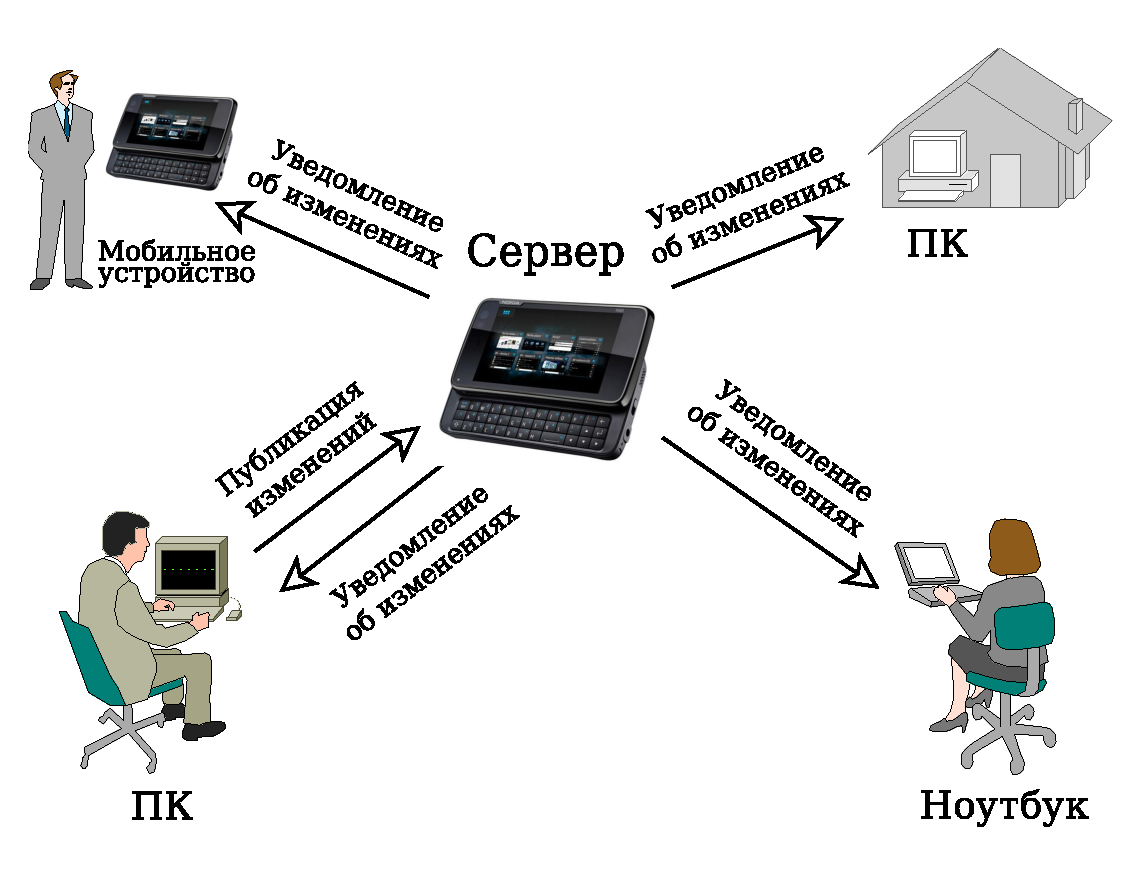
\includegraphics[width=\linewidth]{users_collaboration_example.pdf}
 \caption{Propagation of mind map changeset}
 \label{users_collaboration_example}
 \end{figure} 

 % notification propagation
 First item in the node is placed by the service in the moment of creation. Other
 items are published by participants of collaboration. Every new modification
 published in the node is retransmitted via update notifications to all
 subscribers and the service holder (see fig. \ref{users_collaboration_example}). 
 Service may reject the changeset if there are some defects (e.g. user wants to 
 update mind map node when it was already deleted by another user) and send error
 notification back to the subscriber.

 Protocol design proposes asynchronous propagation of modifications on the client
 side of publish/subscribe interaction. User changes to the mind map in the form
 of XML-serialized command are transmitted to the service and do not store in
 the local undo stack. Only changesets that were received as update notifications
 are added to the stack.

 Subscribers can retrieve all items stored in the node in any time. This
 way clients may synchronize contents of their local copy of mind map if
 transmitted changeset is rejected. Service does not need any additional effort
 to have up-to-date map because all notifications are local and can not be lost
 during transmission.

 To achieve this asynchronous process new element was added to the core of
 HiveMind --- NetworkController. It manages pub/sub protocol handlers. All
 QUndoCommands created as a result of mind map modifications are passed to the
 controller. If there is no network collaboration at the moment command will be
 sent back to MainWindowController and added to the local undo/redo stack.
 Otherwise command will be serialized and send to the service. Update
 notifications are deserialized into QUndoCommands and added to the undo/redo
 stack.

 The drawbacks of current collaboration protocol design and implementation
 include following statements. Client must wait for an update notification in
 order to see changes that he or she made to the shared mind map. Participants
 cannot use undo/redo commands.

 not 4 current document, may be next one
 There are brilliant examples on how to build iterative update shared space -
 Version Control Systems. Their main aim is almost the same as editing shared
 mind map: provide access to common space of source files. VCS can do all the 
 work here, but they do not provide any notification to all people involved in
 collaborative work. They use robust protocols, send only difference between
 committed versions, and do it really slow. \ldots

\section{Реализация контекстного меню узла}\label{sec:context_menu}

\subsection*{Алгоритм анимации меню}

\subsubsection*{Выбор радиусов эллипса}

\subsubsection*{Вычисление координат кнопок}

\section{Реализация редактора текста узла}\label{sec:node_text_editor}

\section{Реализация поддержки пиктограмм в узлах}\label{sec:node_icons_support}
